First we generate a large number of phase realization $\{\theta_i\}_{i=1}^{10^8}$  from uniform distribution $\mathcal{U}(-\pi, \pi)$
\begin{itemize}
    \item[(a)] Given $v = 20$ km/hr and $f_c = 2$GHz, the doppler shift for each $\theta_i$ is obtained by
    \begin{eqnarray*}
        f_{D, i} & = & f_m \cos\left(\theta_i\right) \\
                 & = & \frac{v}{\lambda_c} \cos\left(\theta_i\right) \\
                 & = & \frac{v}{v_c} f_c \cos\left(\theta_i\right) \quad \text{where} \quad v_c = 3 \cdot 10^8 \, m/s
    \end{eqnarray*}
    After calculating doppler shift for each $\theta_i$, we can plot the histogram of $\{f_{D,i}\}$ to see its pdf and cdf.
    \begin{figure}[H]
        \centering
        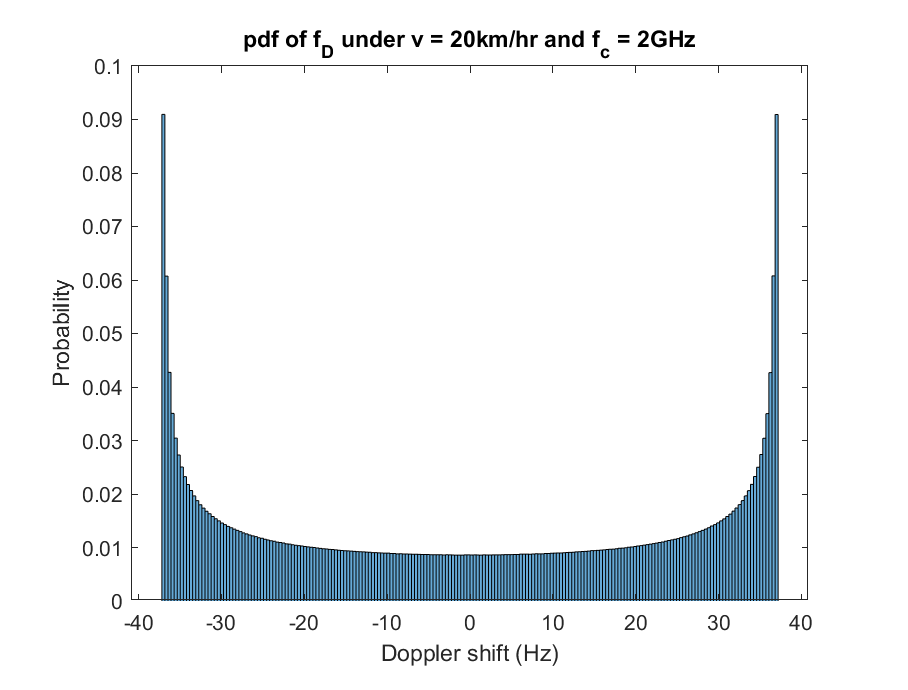
\includegraphics[scale = 0.8]{a_pdf.eps}
    \end{figure}
    \begin{figure}[H]
        \centering
        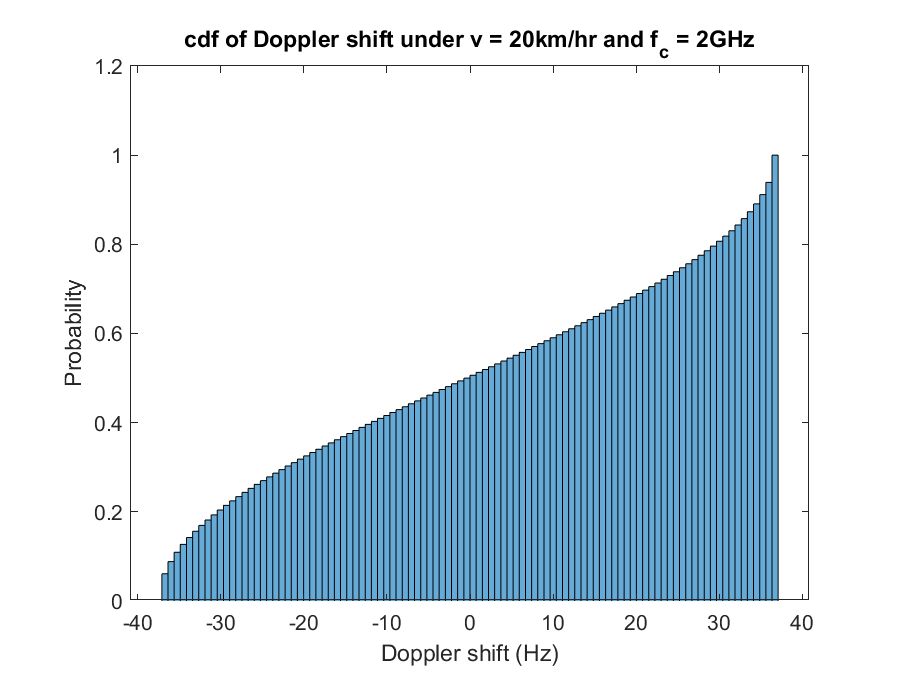
\includegraphics[scale = 0.8]{a_cdf.eps}
    \end{figure}
    \item[(b)] Totally the same as (a), just change $v$ and $f_c$.
    \begin{figure}[H]
        \centering
        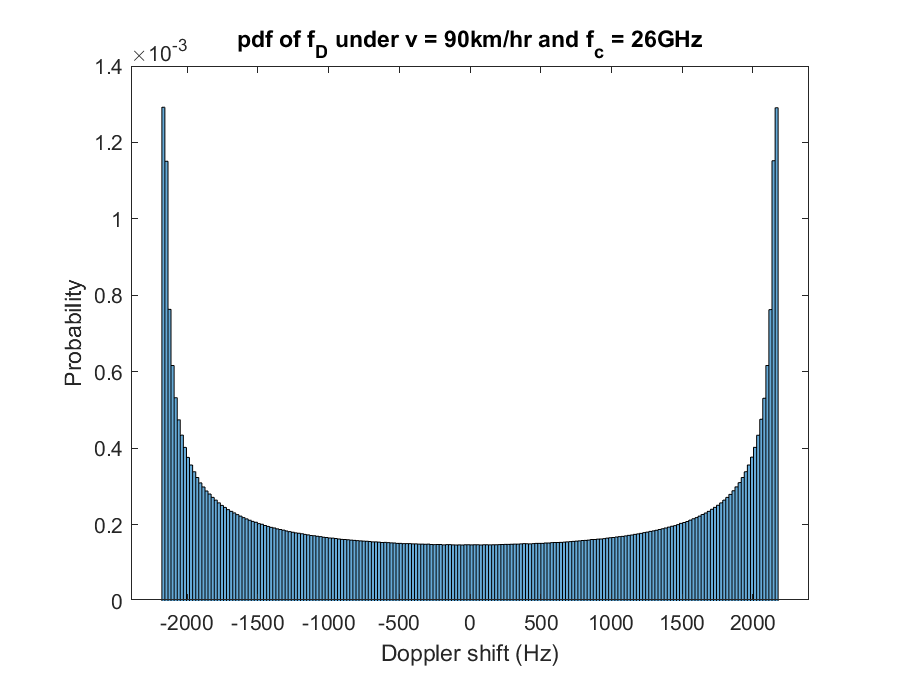
\includegraphics[scale = 0.8]{b_pdf.eps}
    \end{figure}
    \begin{figure}[H]
        \centering
        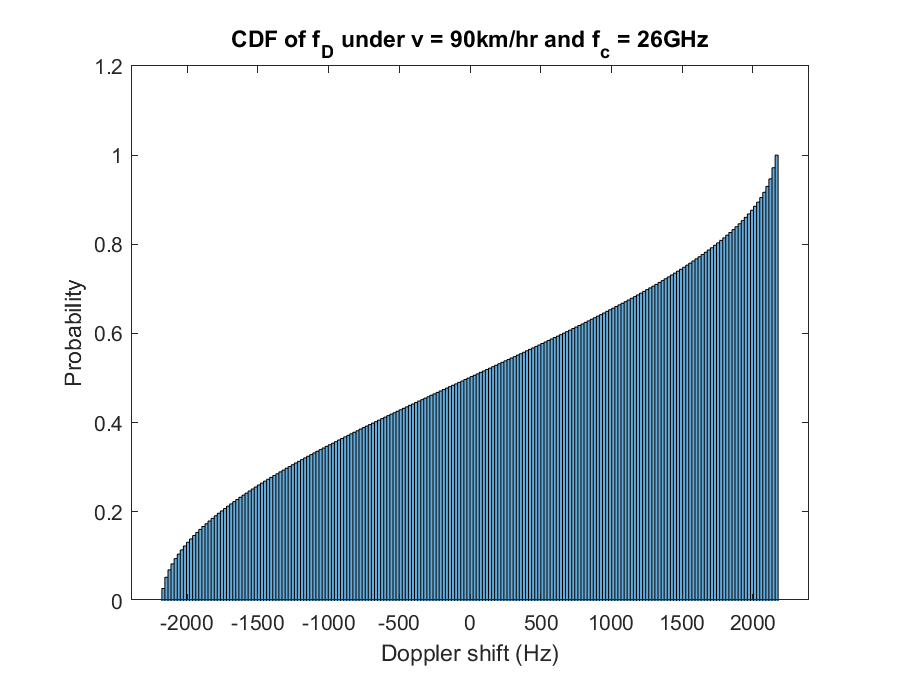
\includegraphics[scale = 0.8]{b_cdf.eps}
    \end{figure}
    \item[(c)] In this part, $v$ also becomes uniform distributed. Hence we generate same number of velocity realization $\{v_i\}_{i=1}^{10^8}$
    and use the same formula to calculate doppler shift for each pair $(v_i, \theta_i)$. 
    \begin{equation*}
        f_{D, i} = \frac{v_i}{v_c} f_c \cos\left(\theta_i\right) \quad \text{where} \quad v_c = 3 \cdot 10^8 \, m/s
    \end{equation*}
    The results are shown below
    \begin{figure}[H]
        \centering
        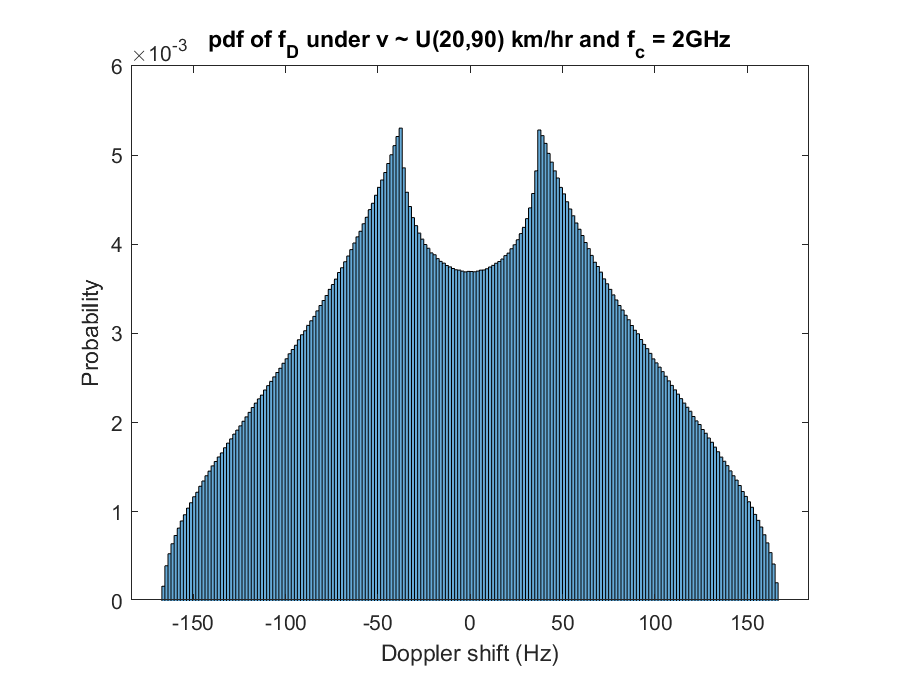
\includegraphics[scale = 0.8]{c_pdf.eps}
    \end{figure}
    \begin{figure}[H]
        \centering
        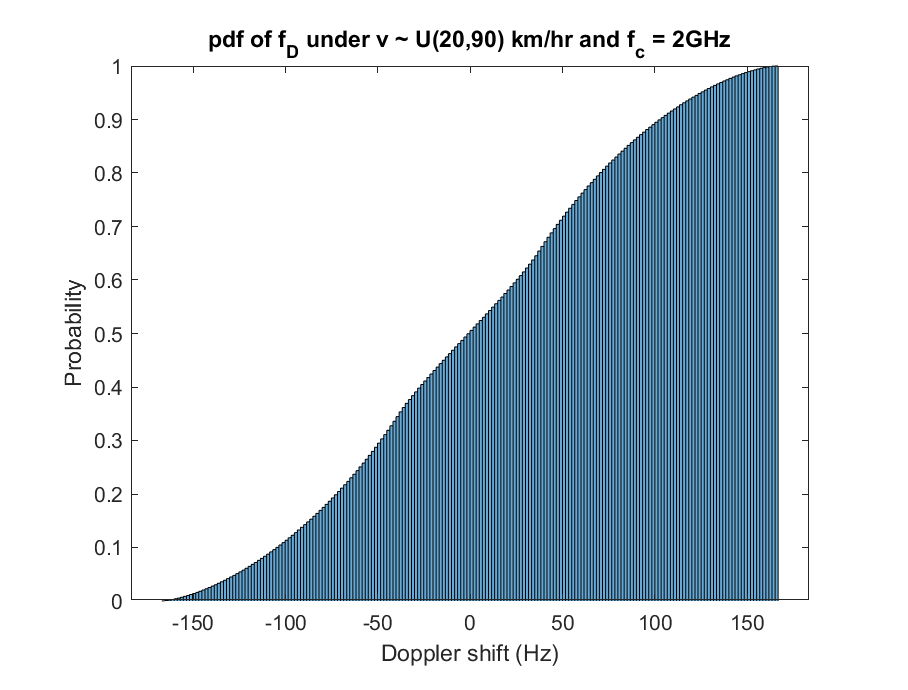
\includegraphics[scale = 0.8]{c_cdf.eps}
    \end{figure}
    \item[(d)] Now, we try to derive the pdf and cdf of $f_D$. Given 
    \begin{eqnarray}
        \theta & \sim & \mathcal{U}(-\pi, \pi) \\
        f_D    &  =   & f_m \cos \left(\theta\right)
    \end{eqnarray}
    For a certain $f_D$, the corresponding solution for (2) is 
    \begin{equation*}
        \theta_1 = \arccos \left(\frac{f_D}{f_m} \right) \quad \text{and} \quad \theta_2 = - \arccos \left(\frac{f_D}{f_m} \right).
    \end{equation*}
    Therefore, the pdf of $f_D$ is then given as
    \begin{eqnarray*}
        P(f_D) & = & \frac{1/2\pi}{\left|-f_m \sin\left(\theta_1\right)\right|} + \frac{1/2\pi}{\left|-f_m \sin\left(\theta_2\right)\right|} \\
               & = & 2 \cdot \frac{1}{2\pi} \cdot \frac{1}{\sqrt{f_m^2 - f_D^2}} \quad \left(\because \sin\left(\arccos \left(\frac{f_D}{f_m} \right)\right) = \frac{\sqrt{f_m^2 - f_D^2}}{f_m} \right)\\
               & = & \frac{1}{\pi} \cdot \frac{1}{\sqrt{f_m^2 - f_D^2}}
    \end{eqnarray*}
    The cdf of $f_D$ can further be derived
    \begin{eqnarray*}
        F(f_D) & = & \int_{-f_m}^{f_D} P(x) \, dx \\
               & = & \frac{1}{\pi \cdot f_m} \int_{-f_m}^{f_D} \frac{1}{\sqrt{1 - \left(\frac{x}{f_m}\right)^{2}}} \, dx \\
               & = & \frac{1}{\pi} \int_{-1}^{\frac{f_D}{f_m}} \frac{1}{\sqrt{1 - u^{2}}} \, du \quad \left(\text{let } u = \frac{x}{f_m}\right) \\
               & = & \frac{1}{\pi} \arcsin \left( u \right) \Bigg|_{-1}^{\frac{f_D}{f_m}} \\
               & = & \frac{1}{\pi} \arcsin\left(\frac{f_D}{f_m}\right) + \frac{1}{2}
    \end{eqnarray*}
    Plot the results with MATLAB, we get
    \begin{figure}[H]
        \centering
        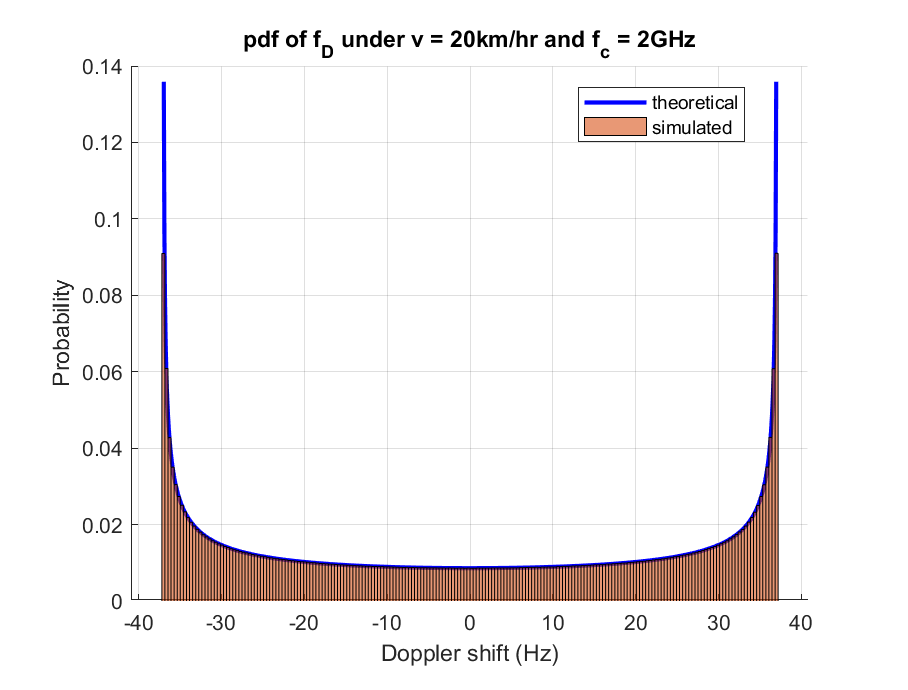
\includegraphics[scale = 0.8]{d_pdf.eps}
    \end{figure}
    \begin{figure}[H]
        \centering
        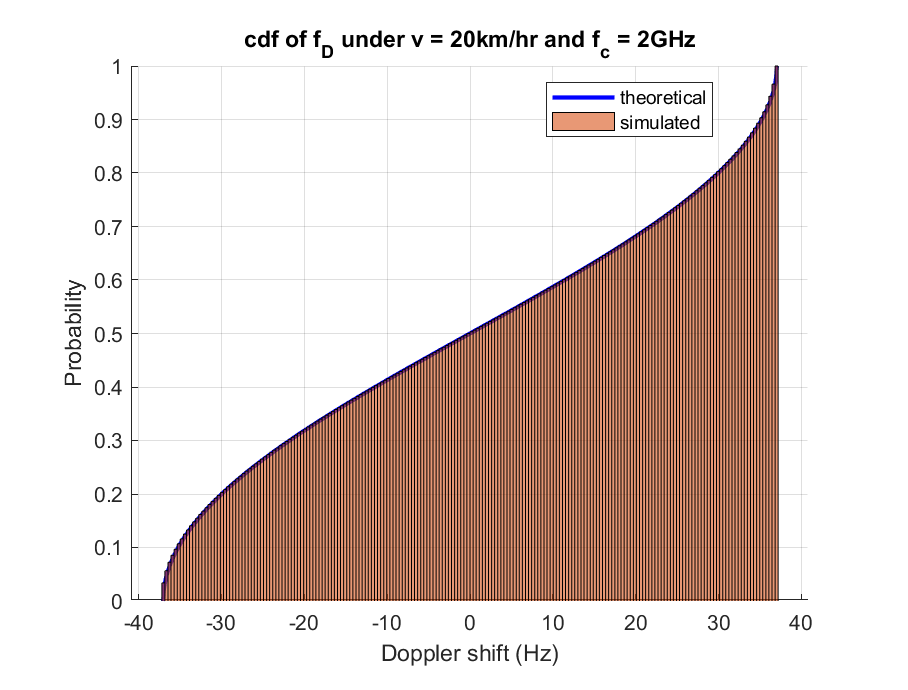
\includegraphics[scale = 0.8]{d_cdf.eps}
    \end{figure}
    The solid line is the theretical result while the histogram is the simulated result. It can be seen that 
    they look similiar.
\end{itemize}